\documentclass{beamer}

\usepackage[T1]{fontenc}
\usepackage{lmodern}
\usepackage{graphicx}
\usepackage{amsmath}
\usepackage{amssymb}
\usepackage{booktabs}
\usepackage{xcolor}
\usepackage{tikz}
\usepackage{array}
\usepackage{colortbl}
\usepackage[authoryear,round]{natbib}
\usepackage{ragged2e}

\usetheme{Madrid}
\usecolortheme{default}
\setbeamertemplate{navigation symbols}{}
\setbeamertemplate{footline}[frame number]
\setbeamersize{text margin left=0.6cm, text margin right=0.6cm}

\definecolor{myprimary}{HTML}{FF9D00}
\definecolor{mysecondary}{HTML}{FF8360}
\definecolor{mydark}{HTML}{243447}
\definecolor{mylight}{HTML}{FFF4E8}
\definecolor{mysoft}{HTML}{F7F7F7}

\setbeamercolor{structure}{fg=myprimary}
\setbeamercolor{title}{fg=white,bg=myprimary}
\setbeamercolor{subtitle}{fg=myprimary}
\setbeamercolor{frametitle}{fg=white,bg=myprimary!90}
\setbeamercolor{block title}{fg=white,bg=myprimary!85}
\setbeamercolor{block body}{fg=black,bg=mylight}
\setbeamercolor{normal text}{fg=mydark,bg=white}
\setbeamercolor{alerted text}{fg=mysecondary}

\setbeamerfont{title}{series=\bfseries,size=\Large}
\setbeamerfont{frametitle}{series=\bfseries,size=\large}
\setbeamerfont{block title}{series=\bfseries}
\setbeamertemplate{bibliography item}[text]
\setlength{\bibsep}{1pt plus 0.2ex}
\bibliographystyle{abbrvnat}

\newcommand{\lerobot}{\texttt{lerobot}}
\newcommand{\lerobotdataset}{\texttt{LeRobotDataset}}
\newcommand{\pizero}{\(\pi_0\)}
\newcommand{\highlight}[1]{\textcolor{myprimary}{\textbf{#1}}}
\newcommand{\statbox}[2]{%
  \begingroup
  \setlength{\fboxsep}{8pt}%
  \colorbox{mylight}{\parbox{\dimexpr\linewidth-2\fboxsep\relax}{\raggedright\textbf{\large #1}\\[-1pt]\small #2}}%
  \endgroup
}

\newcommand{\circled}[1]{%
  \tikz[baseline=(char.base)]\node[draw,circle,inner sep=1pt,thick](char){\textbf{#1}};%
}

\newcommand{\lightbox}[1]{%
  \tikz[baseline=(txt.base)]{
    \node[
      fill=myprimary!15,
      rounded corners=2pt,
      inner xsep=4pt,
      inner ysep=1.5pt
    ] (txt) {\strut #1};
  }%
}

\newcommand{\commonauthors}{%
  Francesco Capuano \and
  Caroline Pascal \and
  Adil Zouitine \and
  Thomas Wolf \and
  Michel Aractingi
}

\newcommand{\shortauthors}{%
  Francesco Capuano, Caroline Pascal, Adil Zouitine, Thomas Wolf, Michel Aractingi
}

\newcommand{\chaptertitleframe}[1]{%
  \begin{frame}[plain]
    \vspace{0.35cm}
    \begin{center}
      \begin{beamercolorbox}[wd=0.86\paperwidth,rounded=true,sep=10pt,center]{title}
        \usebeamerfont{title}\inserttitle
      \end{beamercolorbox}

      \vspace{0.55cm}
      {\Large\bfseries\textcolor{myprimary}{\insertsubtitle}\par}
      \vspace{0.15cm}
      {\small\color{mydark}\shortauthors\par}

      \vspace{0.45cm}
      
\includegraphics[height=1.0cm]{hf.pdf}
      \hspace{0.45cm}
      
\includegraphics[height=0.95cm]{oxford_logo.png}

      \vspace{0.55cm}
      \begin{beamercolorbox}[wd=0.8\paperwidth,rounded=true,sep=8pt,center]{block body}
        \small #1
      \end{beamercolorbox}
    \end{center}
  \end{frame}
}

\newcommand{\sources}[1]{%
  \vfill
  {\raggedright\tiny\color{black!65}\textbf{Refs:} #1\par}
}

\graphicspath{{../../../figures/}{../../../logos/}}

\title[Robot Learning Tutorial]{Robot Learning: A Tutorial}
\subtitle{Chapter 1: Introduction}
\author[Capuano et al.]{\commonauthors}
\date{}
\titlegraphic{
  \vspace{-1.1cm}
  
\includegraphics[height=1.4cm]{hf.pdf}
  \hspace{0.3cm}
  
\includegraphics[height=1.2cm]{oxford_logo.png}
}

\begin{document}

\chaptertitleframe{Why robot learning matters now, how \lerobot{} structures the stack, and how the rest of the tutorial is organized.}

\begin{frame}{Why Robot Learning Now?}
  \begin{itemize}
    \item Robotics is still constrained by \highlight{engineering-heavy pipelines}, brittle modeling assumptions, and expensive hardware integration.
    \item Modern ML offers a different route: \highlight{learn perception-to-action mappings} from interaction data instead of specifying every component by hand.
    \item The tutorial's stance is intentionally hybrid:
    \item Classical robotics remains essential, but \highlight{learning is increasingly the right abstraction} for multimodal, unstructured, real-world tasks.
  \end{itemize}

  \vspace{0.2cm}
  \statbox{Working thesis}{Robot learning matters because it can reduce modeling burden, absorb richer sensory inputs, and benefit directly from the growing supply of open robotics data.}
\end{frame}

\begin{frame}{Tutorial Map}
  \begin{columns}[T,onlytextwidth]
    \begin{column}{0.5\textwidth}
      \begin{enumerate}
        \item \highlight{Introduction}: why the field is shifting
        \item \highlight{Classical Robotics}: what explicit models buy us
        \item \highlight{Reinforcement Learning}: learning through interaction
      \end{enumerate}
    \end{column}
    \begin{column}{0.5\textwidth}
      \begin{enumerate}
        \setcounter{enumi}{3}
        \item \highlight{Imitation Learning}: learning from demonstrations
        \item \highlight{Generalist Policies}: foundation-style robotics models
      \end{enumerate}
    \end{column}
  \end{columns}

  \vspace{0.4cm}
  \statbox{Exposition strategy}{Each chapter moves from intuition to concrete mechanisms to practical use in \lerobot.}
\end{frame}

\begin{frame}{\lerobot~at a Glance}
  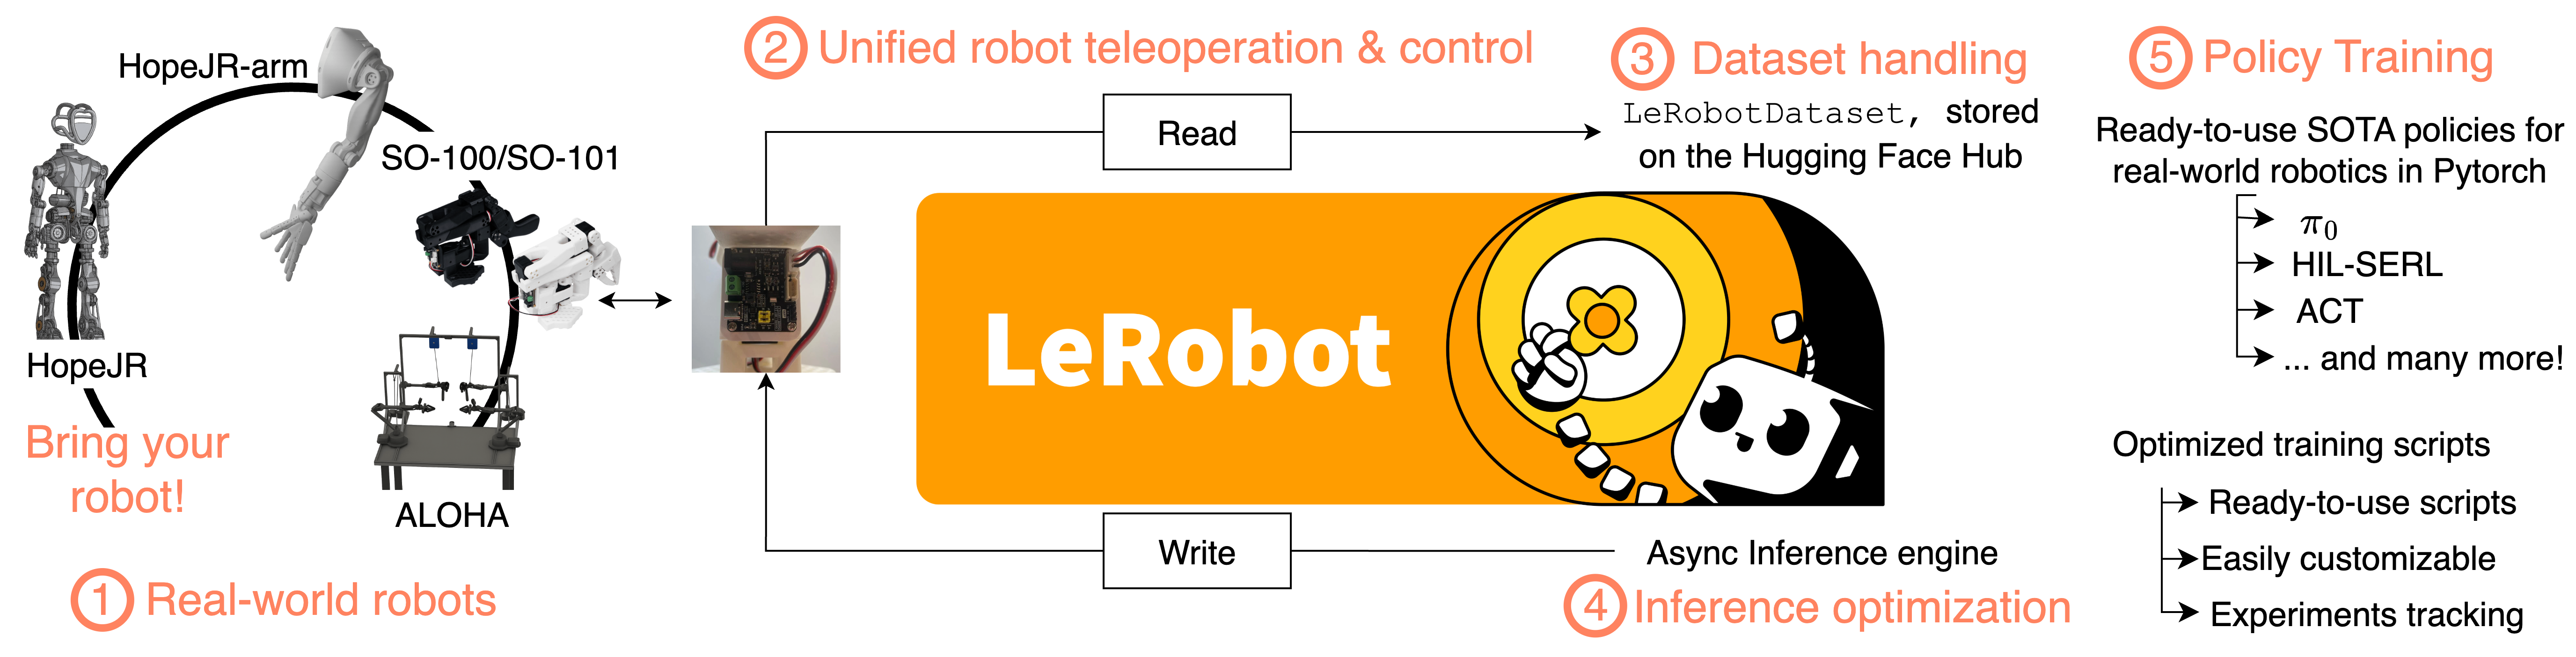
\includegraphics[width=\linewidth,height=0.72\textheight,keepaspectratio]{ch1/ch1-lerobot-figure1.png}
  \begin{itemize}
    \item \lerobot~is positioned as an \highlight{end-to-end open-source stack} for robot learning.
    \item The stack spans hardware interfaces, datasets, training, and deployment.
  \end{itemize}
\sources{\citep{cadeneLeRobotStateoftheartMachine2024}}
\end{frame}

\begin{frame}{What the Stack Needs to Provide}
  \begin{columns}[T,totalwidth=\textwidth]
    \begin{column}{0.25\textwidth}
      \centering
      \textbf{\circled{1} Robots} \\
      \vspace{0.8em}
      Support affordable real robots and expose a \highlight{common low-level interface}.
    \end{column}
    \begin{column}{0.25\textwidth}
      \centering
      \textbf{\circled{2} Data} \\
      \vspace{0.8em}
      Standardize multimodal trajectories so collection and reuse are \highlight{easy at scale}.
    \end{column}
    \begin{column}{0.25\textwidth}
      \centering
      \textbf{\circled{3} Policies} \\
      \vspace{0.8em}
      Provide reference implementations for \highlight{RL, BC, and VLA} methods.
    \end{column}
    \begin{column}{0.25\textwidth}
      \centering
      \textbf{\circled{4} Runtime} \\
      \vspace{0.8em}
      Separate action planning from execution to keep \highlight{deployment responsive}.
    \end{column}
  \end{columns}
\end{frame}

\begin{frame}{Why Data Infrastructure Matters}
  \begin{itemize}
    \item Robot learning is increasingly bottlenecked by \highlight{data usability}, not just by model design.
    \item Trajectories must combine proprioception, images, actions, timing, tasks, and embodiment metadata.
    \item The same dataset should support:
    \item offline BC training, replay-buffer style RL workflows, and model sharing across the community.
  \end{itemize}

  \vspace{0.25cm}
  \statbox{\lerobotdataset}{The dataset format is treated as a first-class part of the robot learning stack, not as an afterthought around a model.}
\end{frame}

\begin{frame}{How \lerobotdataset~Is Organized}
  \begin{columns}[T,onlytextwidth]
    \begin{column}{0.33\textwidth}
      \textbf{Tabular data}
      \begin{itemize}
        \item joint states
        \item actions
        \item memory-mapped parquet storage
      \end{itemize}
    \end{column}
    \begin{column}{0.33\textwidth}
      \textbf{Visual data}
      \begin{itemize}
        \item camera streams
        \item MP4 episode chunks
        \item grouped by view
      \end{itemize}
    \end{column}
    \begin{column}{0.33\textwidth}
      \textbf{Metadata}
      \begin{itemize}
        \item schema and stats
        \item tasks and episode boundaries
        \item versioning and fps
      \end{itemize}
    \end{column}
  \end{columns}

  \vspace{0.35cm}
  \statbox{Design principle}{Separate efficient storage from the user-facing API so large datasets stay scalable without becoming cumbersome to use.}
\end{frame}

\begin{frame}{Training-Time Ergonomics}
  \begin{itemize}
    \item Policies rarely consume a single frame in isolation.
    \item RL often needs \highlight{histories of observations}; BC often predicts \highlight{chunks of future actions}.
    \item \lerobotdataset~supports native windowing with padding and masks, so higher-level code can stay simple.
    \item Streaming mode makes large Hub-hosted datasets usable without local full copies.
  \end{itemize}

  \vspace{0.2cm}
  \statbox{Practical consequence}{The same dataset abstraction can power local batching, streamed training, and downstream PyTorch loaders with minimal code changes.}
\end{frame}

\begin{frame}{Practical Workflow in \lerobot}
  \begin{block}{Dataset consumption}
    Load a dataset, define observation/action windows, and batch with a standard \texttt{DataLoader}.
  \end{block}

  \begin{block}{Dataset recording}
    Use the collection utilities to store synchronized sensorimotor streams and task metadata in the same format.
  \end{block}

  \begin{itemize}
    \item Reference snippets: \texttt{snippets/ch1/01\_datasets.py} and \texttt{snippets/ch1/02\_record\_data.py}
    \item The point is not just convenience: it is \highlight{standardization across collection, training, and sharing}.
  \end{itemize}
\end{frame}

\begin{frame}{What This Introduction Sets Up}
  \begin{itemize}
    \item Classical robotics explains why explicit modeling has been so successful.
    \item RL explains how interaction-driven learning replaces parts of that stack.
    \item Imitation learning explains why demonstrations can be safer and more practical than reward design.
    \item Generalist policies explain how scale, language, and shared architectures are changing the frontier.
  \end{itemize}

  \vspace{0.25cm}
  \statbox{Key takeaway}{The rest of the tutorial is best read as a progression from structured control pipelines toward data-centric, increasingly general robot policies.}
\end{frame}

\begin{frame}[allowframebreaks]{Selected References}
\scriptsize
\nocite{bekrisStateRobotMotion2024,koberReinforcementLearningRobotics,zhaoLearningFineGrainedBimanual2023,black$p_0$VisionLanguageActionFlow2024,shukorSmolVLAVisionLanguageActionModel2025}
\bibliography{../shared/references}
\end{frame}

\end{document}
